% =====================================================================================================
\section{Hardware Results}\label{sec:hwresults}
\subsection{Cycles and throughput}
% generated by paper/make_assets.py from paper/data -- do not edit
\begin{table}[t]
\caption{Encoder cycles per frame in RTL simulation (160x128, 100\,MHz). The last column extrapolates to 640$\times$480 at the same cycles per pixel.}
\label{tab:cycles}
\centering\small
\resizebox{\columnwidth}{!}{%
\begin{tabular}{lrrrr}
\toprule
Mode & Cycles & Cycles/pixel & $\Delta$ vs E0 & fps (640$\times$480) \\
\midrule
E0 & 33519 & 1.637 & +0 & 199 \\
E1 & 33518 & 1.637 & -1 & 199 \\
E2 & 33521 & 1.637 & +2 & 199 \\
E3 & 33518 & 1.637 & -1 & 199 \\
E4 & 33519 & 1.637 & +0 & 199 \\
\bottomrule
\end{tabular}}
\end{table}

In RTL simulation of a 160$\times$128 frame, the cycle counts of E0--E4 differ by at most \MaxExtraCycles{} cycles (Table~\ref{tab:cycles}), which is handshake noise rather than encryption work: as Proposition~\ref{prop:supply} predicts, encryption costs no cycles. Above the floor of 1.5 cycles per pixel, the only cost is filling the first MCU row: on \NumScaleSizes{} frame sizes the RTL follows~\eqref{eq:fill}, \CyclesPerPixel{} cycles per pixel at 160$\times$128 and \CppVGA{} at 640$\times$480 (Fig.~\ref{fig:throughput}).

\begin{figure}[t]
\centering
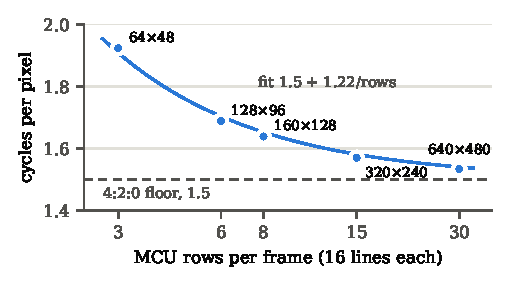
\includegraphics[width=\columnwidth]{figures/fig_throughput.pdf}
\caption{Cycles per pixel of the encoder RTL against frame height, measured in cycle-accurate simulation (dots), with the fitted law $1.5+\FillA/r$ of~\eqref{eq:fill} for $r$ MCU rows.}
\label{fig:throughput}
\end{figure}

\begin{figure}[t]
\centering
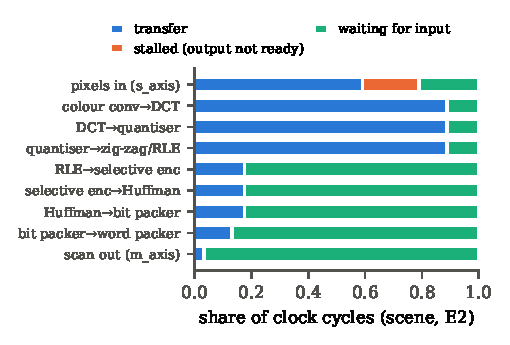
\includegraphics[width=\columnwidth]{figures/fig_stall.pdf}
\caption{Where the clock cycles go: share of cycles in which each handshake of the encoder pipeline transfers data, is stalled by its consumer, or waits for its producer (RTL simulation, synthetic scene, E2). Everything after the run-length coder, including the cipher, idles most of the time.}
\label{fig:stall}
\end{figure}
\textit{Where the cycles go.} Monitoring every handshake of the RTL pipeline over \ProfileCases{} cases (three images, three levels) shows the same cycles per pixel to within \ProfileCppSpread{} for every image and level, and an entropy path (run-length coding, encryption, Huffman coding, packing) that waits for data at least \EntropyIdle\,\% of the time (Fig.~\ref{fig:stall}). Faster designs must therefore widen the transform path, not the cipher, which is what the lanes do.

\textit{Lanes.} Measured at 100\,MHz on 640$\times$480 frames, bit-exact for every frame (Fig.~\ref{fig:lanesrtl}), one, two and four lanes reach \RtlOneLaneMpix, \RtlTwoLanesMpix{} and \RtlFourLanesMpix\,Mpixel/s (\RtlOneLaneCpp, \RtlTwoLanesCpp{} and \RtlFourLanesCpp{} cycles per pixel), against the bounds \BoundOneMpix, \BoundTwoMpix{} and \BoundFourMpix{} of~\eqref{eq:lanes}. Four lanes give \RtlFourLanesSpeedup$\times$ the single pipeline, \RtlFourLanesFps{} frames/s at 640$\times$480 or \RtlFourLanesHdFps{} at 1080p, above the \mbox{150\,Mpixel/s} that the commercial encoder of~\cite{logijpge} reports at 150\,MHz without any cryptography, at two thirds of its clock. The gap to the bound has two causes: a frame starts only after the previous one is done, so every frame pays~\eqref{eq:fill} once, and each segment adds a keystream restart and a byte flush. An event model that also lets the next frame's first MCU row arrive early projects \ProjTwoLanesMpix{} and \ProjFourLanesMpix\,Mpixel/s (Fig.~\ref{fig:lanes}). The latency from the first pixel to the first scan word is \RtlFourLanesLatUs\,$\mu$s (\RtlFourLanesLatLines{} lines of a 640$\times$480 frame) for any number of lanes: the 16 lines of the first MCU row plus the pipeline. E5, with one restart per MCU, costs a few per cent of throughput in the lane encoder. Two build options trade along other axes. With camera-native YUYV input (four pixels per beat, Section~\ref{sec:lanes}) four lanes reach \YuyvFourLanesMpix\,Mpixel/s (\YuyvFourLanesCpp{} cycles per pixel) and read \YuyvFourLanesInMBs\,MB/s from DDR instead of \RtlFourLanesInMBs; with one line-buffer set per lane instead of two, four lanes keep \NbufOneFourLanesMpix\,Mpixel/s (\NbufOneFourLanesCpp{} cycles per pixel) on half the converter memory, which is what lets four lanes take 1080p lines on this device.

\begin{figure}[t]
\centering
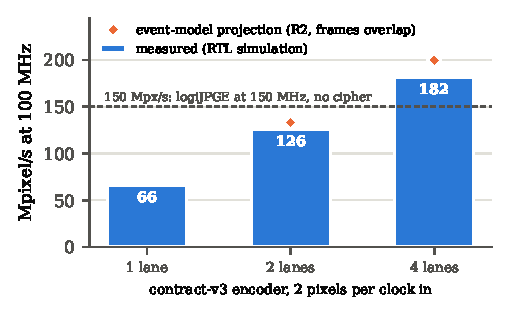
\includegraphics[width=\columnwidth]{figures/fig_lanes_rtl.pdf}
\caption{Throughput of the lane encoder, 640$\times$480 frames at 100\,MHz, measured in cycle-accurate simulation with every frame bit-exact against the golden model (bars), next to the event-model projection with overlapping frames (diamonds) and the published figure of a commercial encoder without cryptography~\cite{logijpge} (dashed).}
\label{fig:lanesrtl}
\end{figure}
\begin{figure}[t]
\centering
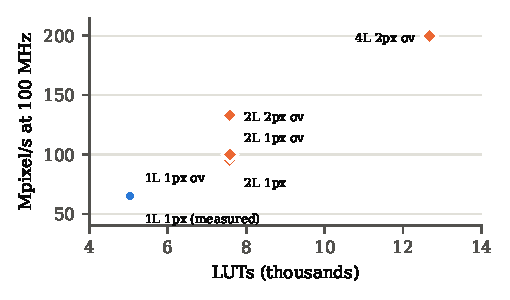
\includegraphics[width=\columnwidth]{figures/fig_lanes.pdf}
\caption{Projected throughput at 100\,MHz against LUTs for 640$\times$480 frames (event model calibrated on the measured RTL law). Labels: $L$ lanes, pixels per clock at the input, ``ov'': the next frame overlaps the current one; the circle is the measured single pipeline.}
\label{fig:lanes}
\end{figure}

\subsection{Area, timing and power}
% generated by paper/make_assets.py from paper/data -- do not edit
\begin{table}[t]
\caption{Resources on the xc7z020 (53\,200 LUT, 106\,400 FF, 140 BRAM36, 220 DSP). Source: Vivado post-route, out of context, 100\,MHz with I/O delays of 20\,\% of the period, WNS +1.524\,ns.}
\label{tab:resources}
\centering\small
\resizebox{\columnwidth}{!}{%
\begin{tabular}{lrrrr}
\toprule
Block & LUT & FF & BRAM36 & DSP \\
\midrule
Encoder (all) & 5043 (9.5\%) & 3506 (3.3\%) & 25.5 (18.2\%) & 23 (10.4\%) \\
\quad colour conversion + line buffers & 409 & 346 & 25 & 0 \\
\quad DCT and quantizer & 808 & 69 & 0 & 22 \\
\quad zig-zag, Huffman, packing & 1030 & 549 & 0 & 0 \\
\quad keystream generator (Ascon) & 874 & 857 & 0 & 0 \\
\quad tag unit (Ascon) & 1357 & 1072 & 0 & 0 \\
\quad selective encryption & 147 & 120 & 0 & 0 \\
\quad AXI-Lite registers & 393 & 452 & 0 & 0 \\
\bottomrule
\end{tabular}}
\end{table}

After place and route in Vivado the single-pipeline encoder meets \TopMhz\,MHz on the xc7z020 (WNS $+$\TopWns\,ns, out of context, I/O delays of 20\,\% of the period), i.e.\ \TopMpix\,Mpixel/s or \FpsVGA{} frames/s at 640$\times$480. Table~\ref{tab:resources} gives the resources (\TopLuts{} LUTs, \TopLutPct\,\% of the device). The two Ascon instances take \CryptoLutShare\,\% of the LUTs; the selective-encryption stage itself is tiny; all \ConvBram{} BRAM36 are the converter's line buffers for 2048-pixel lines. With switching activity from simulating a real frame (SAIF), the encoder draws about \SaifTopMw\,mW; the vectorless estimate is \TopPowerMw\,mW. Two lanes take \TwoLanesLuts{} LUTs, \TwoLanesBram{} BRAM36 and \TwoLanesDsp{} DSPs (WNS $\TwoLanesWns$\,ns), four lanes \FourLanesLuts{} LUTs, \FourLanesBram{} BRAM36 and \FourLanesDsp{} DSPs (WNS $\FourLanesWns$\,ns, lines up to 1024 pixels). E5 adds no BRAM or DSP; with two lanes it draws \SaifLanesEfiveMw\,mW against \SaifLanesEtwoMw\,mW for E2. Out of context one, two and four lanes also meet 150\,MHz (WNS \TopWnsAtOneFifty, \LanesTwoWnsAtOneFifty{} and \LanesFourWnsAtOneFifty\,ns, Section~\ref{sec:hardware}); at that clock four lanes give \LanesFourFastMpix\,Mpixel/s from their cycle count. The complete PYNQ-Z2 systems all close timing: the single pipeline at \OverlayMhz\,MHz with \OverlayLuts{} LUTs (WNS $\OverlayWns$\,ns), two lanes on a 64-bit pixel stream at \OverlayLanesMhz\,MHz with \OverlayLanesLuts{} LUTs (WNS $\OverlayLanesWns$\,ns), and four lanes at \OverlayLanesFourMhz\,MHz with \OverlayLanesFourLuts{} LUTs, \OverlayLanesFourBram{} BRAM36 and \OverlayLanesFourDsp{} DSPs (WNS $\OverlayLanesFourWns$\,ns, \OverlayLanesFourLutPct\,\% of the LUTs). The same four lanes with lines up to 2048 pixels (one line-buffer set per lane, for 1080p) and with camera-native YUYV input also close at \OverlayLanesFourHdMhz{} and \OverlayLanesFourYuyvMhz\,MHz (WNS $\OverlayLanesFourHdWns$ and $\OverlayLanesFourYuyvWns$\,ns). For attacks on the board, a variant of the two-lane system places a fault injector between the encoder and the receive DMA, after the tag is computed, which flips one non-marker bit of the scan on a trigger; it closes at \OverlayTamperMhz\,MHz (WNS $\OverlayTamperWns$\,ns), and the injector takes \TamperInjLuts{} LUTs. Vivado estimates \OverlayPowerW, \OverlayLanesPowerW{} and \OverlayLanesFourPowerW\,W for the complete systems, dominated by the processing system. At \OverlayLanesFourMhz\,MHz the four lanes' cycle count gives \SysFourLanesMpix\,Mpixel/s (\SysFourLanesFps{} frames/s at 640$\times$480; this system takes lines up to 1024 pixels), more than the 150\,Mpixel/s of the fastest published Zynq-7020 encoder, which has no cipher (Table~\ref{tab:compare}); on the board the encoding clocks give the same \BdFourBusyMpix\,Mpixel/s (Section~\ref{sec:board}).

% generated by paper/make_assets.py from paper/data -- do not edit
\begin{table}[t]
\caption{Comparison with published FPGA designs. Their numbers are as reported by each source; ours are
post-route (Table~\ref{tab:resources}) with throughput from the RTL cycle count of a 640$\times$480 frame. Mpx/s: million pixels per second. Lanes (v3): throughput in RTL simulation at 100\,MHz, area post-route; board: the complete PYNQ-Z2 design (processing system, DMA, 4 lanes) measured on the board, encoder time of a 640$\times$480 frame from its cycle counter.\ifextended{} Kishore et al.: Stratix~IV ALUTs and 18-bit multipliers, 256$\times$256 grey images; Ba\u{g}baba and \"Ors report no throughput.\fi}
\label{tab:compare}
\centering\small
\resizebox{\columnwidth}{!}{%
\begin{tabular}{llrrrrrl}
\toprule
Design & Device & LUT & BRAM & DSP & MHz & Mpx/s & Crypto \\
\midrule
Ours: encoder & Zynq-7020 & 5{,}043 & 25.5 & 23 & 100 & 65 & sel.\ AEAD \\
Ours: encoder & Zynq-7020 & 5{,}126 & 25.0 & 23 & 150 & 98 & sel.\ AEAD \\
Ours: one Ascon & Zynq-7020 & 743--970 & 0 & 0 & 100 & -- & AEAD core \\
\ifextended Ours: 2 lanes (v3) & Zynq-7020 & 10{,}099 & 52.0 & 46 & 100 & 126 & sel.\ AEAD \\ \fi
Ours: 4 lanes (v3) & Zynq-7020 & 17{,}515 & 56.0 & 92 & 100 & 182 & sel.\ AEAD \\
Ours: 4 lanes (v3) & Zynq-7020 & 17{,}887 & 54.0 & 92 & 150 & 272 & sel.\ AEAD \\
Ours: 4 lanes, board & Zynq-7020 & 20{,}123 & 58.5 & 92 & 125 & 156 & sel.\ AEAD \\
logiJPGE~\cite{logijpge} & Zynq-7020 & 3{,}240 & 16 & 30 & 150 & 150 & none \\
CAST JPEG-E-S~\cite{castjpeg} & Artix-7 & 3{,}069 & 2 & 16 & 166 & -- & none \\
Khairallah~\cite{khairallah2023} & Artix-7 & 1{,}031 & 0 & 0 & 200 & -- & MAC \\
Kurian~\cite{kurian2025} & Artix-7 & 5{,}335 & 32 & 0 & 100 & -- & AEAD \\
\ifextended Kishore~\cite{kishore2015} & Stratix IV & 2{,}250 & -- & 47 & 100 & 11.1 & scrambling \\ \fi
\ifextended Ba\u{g}baba~\cite{bagbaba2015} & Virtex-6 & 2{,}130 & -- & 9 & 87 & -- & TEA \\ \fi
\bottomrule
\end{tabular}}
\end{table}

% generated by paper/make_assets.py from paper/data -- do not edit
\begin{table}[t]
\caption{Hardware figures of merit at 100\,MHz, 640$\times$480, E2: throughput from cycle-accurate RTL simulation (no DMA stalls), area and power post-route. Energy per pixel = on-chip power / throughput.}
\label{tab:hweff}
\centering\small\setlength{\tabcolsep}{2.5pt}
\resizebox{\columnwidth}{!}{%
\resizebox{\columnwidth}{!}{%
\begin{tabular}{lrrrrrrr}
\toprule
Design & LUT & Mpx/s & Mpx/s per kLUT & Gbit/s in & fps 1080p & Power (mW) & nJ/pixel \\
\midrule
Ours{,} single pipeline (v2) & 4{,}752 & 65 & 13.7 & 1.56 & 31 & 205 (SAIF) & 3.15 \\
Ours{,} 2 lanes & 9{,}394 & 126 & 13.4 & 3.03 & 61 & 322 (SAIF) & 2.55 \\
Ours{,} 4 lanes & 16{,}098 & 182 & 11.3 & 4.36 & 88 & 549 (vectorless) & 3.02 \\
\bottomrule
\end{tabular}}}
\end{table}


\subsection{Comparison}
Table~\ref{tab:compare} sets the design against published FPGA work. Each of our Ascon cores (\AsconLutMin--\AsconLutMax{} LUTs) is as small as the round-per-cycle Ascon-p cores of~\cite{khairallah2023}; our JPEG datapath without the cipher (colour conversion, transform, quantizer and entropy coder in Table~\ref{tab:resources}) uses fewer LUTs than the commercial encoders~\cite{logijpge,castjpeg}, which however process one sample per clock at 150--166\,MHz with less block RAM and no cryptography. Table~\ref{tab:hweff} gives the figures of merit that hardware papers compare: \HeTopPerKlut, \HeTwoPerKlut{} and \HeFourPerKlut\,Mpixel/s per thousand LUTs for one, two and four lanes, against \HeKishorePerKlut{} for the scrambling encoder of Kishore et al.~\cite{kishore2015} and \HeLogiPerKlut{} for the commercial encoder without cryptography~\cite{logijpge}; and, from Vivado's power estimate rather than a measurement, \HeTopNj, \HeTwoNj{} and \HeFourNj\,nJ per pixel. One Ascon core accepts a 128-bit block every \AsconCyclesPerBlock{} clocks once initialized (eight rounds and one handshake, measured in RTL), i.e.\ \AsconGbps\,Gbit/s at 100\,MHz or \AsconGbpsPerKlut\,Gbit/s per thousand LUTs of the larger instance; the selective encryption needs far less, since it consumes at most one sign bit and the amplitude bits of each non-zero coefficient. The lanes buy throughput, not efficiency: each lane carries its own transform and line buffers, so area grows with $L$ while the energy per pixel stays roughly constant.

\subsection{Board evaluation}\label{sec:board}
% generated by paper/make_assets.py from paper/data -- do not edit
\begin{table*}[t]
\caption{On the PYNQ-Z2 (24 Oct 2026): the final board images, each at the clock it was built for, and the same
function on the board's ARM Cortex-A9. Bit-exact: every frame of every level compared byte for byte (scan and tag)
with the golden model running on the board (58 frames in all). Fabric: START to DONE from
the encoder's CYCLES register for one 640$\times$480 frame (Mpixel/s in brackets); wait: share of those cycles in
which the encoder could take a pixel but the DMA had none, mostly because the Python driver starts the DMA after the encoder. Frame: a complete authenticated JPEG with headers (and
for E5 the segment order) on the ARM, the pixels already in the DMA buffer as a camera would leave them, median of
50 frames (frames/s in brackets). ARM rows: median of 30 frames; ``file'' encrypts the whole JPEG, so it does not
play without the key.}
\label{tab:board}
\centering\small\setlength{\tabcolsep}{4pt}
\resizebox{\textwidth}{!}{%
\begin{tabular}{lrlrrrr}
\toprule
Encoder & MHz & Bit-exact & Fabric, ms & Wait (\%) & E2 frame, ms & E5 frame, ms \\
\midrule
4 lanes & 125 & E0--E5 & 1.97 (156) & 31 & 5.9 (169) & 8.4 (119) \\
2 lanes & 100 & E0--E5 & 3.06 (100) & 21 & 7.0 (144) & 9.8 (102) \\
1 lane & 100 & E0--E4 & 5.34 (58) & 12 & 9.2 (108) & -- \\
\midrule
ARM, ours in C, 1 core & -- & E0--E5 & -- & -- & 114.2 (8.8) & 133.0 (7.5) \\
ARM, ours in C, 2 cores & -- & E0--E5 & -- & -- & 61.6 (16.2) & 74.8 (13.4) \\
ARM, libjpeg-turbo, no security & -- & -- & -- & -- & 28.8 (34.8) & -- \\
ARM, libjpeg-turbo + Ascon (file) & -- & -- & -- & -- & 31.7 (31.5) & -- \\
ARM, libjpeg-turbo + AES-GCM (file) & -- & -- & -- & -- & 31.9 (31.3) & -- \\
\bottomrule
\end{tabular}}
\end{table*}

\begin{figure}[t]
\centering
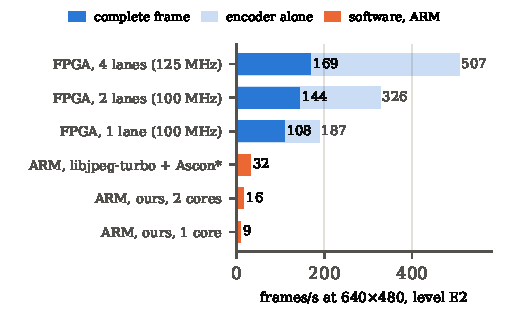
\includegraphics[width=\columnwidth]{figures/fig_board_fps.pdf}
\caption{Measured on the PYNQ-Z2: authenticated 640$\times$480 frames per second (E2) of the three board images, each at the clock it was built for, and of software on the board's two Cortex-A9 cores (Table~\ref{tab:board}). Light: the encoder alone, START to DONE from its cycle counter. *Encrypts the whole file, so it does not play without the key.}
\label{fig:boardfps}
\end{figure}
\begin{figure}[t]
\centering
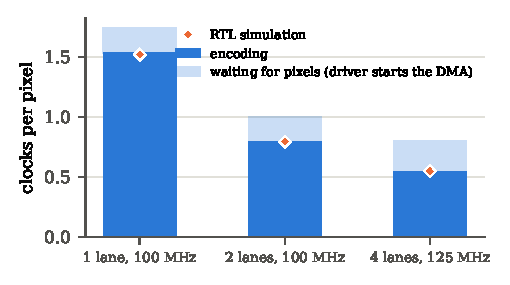
\includegraphics[width=\columnwidth]{figures/fig_board_cycles.pdf}
\caption{Where the fabric's clocks go on the board, per pixel of a 640$\times$480 frame (E2): encoding, and waiting for pixels, almost all of it because the Python driver starts the DMA after the encoder. Diamonds: the cycle count of the same RTL in simulation.}
\label{fig:boardcycles}
\end{figure}
Following the practice of Section~\ref{sec:evalpractice}, the board evaluation on the PYNQ-Z2 has four parts, all scripted and rehearsed beforehand against an emulation of the bitstream: (A1) a bit-exact gate that encodes frames of two sizes in every level on the fabric and compares every byte and tag with the golden model running on the board; (A2) the fabric's own time from its cycle counters and the time of a complete frame; (A3) the same function on the board's processing system: our encoder compiled in C for the Cortex-A9, gated bit-exact against the golden model in every level and run on one and both cores (contract-v3 segments are independent, so the two cores act like two lanes), next to libjpeg-turbo alone and with whole-file Ascon-AEAD128 or AES-GCM, the fair baseline because that core has no AES instructions; and (A4) energy per frame. Table~\ref{tab:board} gives the results of the board day, each image at the clock it was built for.

\textit{Correctness (A1).} All \BdImages{} board images, one, two and four lanes, are bit-exact with the golden model in every level they implement: \BdFramesTotal{} frames, every scan byte and every tag, after the \BoardFramesTotal{} frames of an earlier two-lane image (rebuilt after one defect in the block design: the DMA's write master was left unconnected; Table~\ref{tab:bugs} lists the lesson). The board thus confirms Lemma~\ref{lem:format} and the lane, E5 and tag logic on silicon, not only in simulation.

\textit{Speed (A2).} The board images count the clocks from START to DONE and, among them, the clocks in which the encoder could take a pixel but the DMA had none (Table~\ref{tab:regs}). Without those waits the counts equal the RTL simulation to within \BdBusyVsRtlMaxPct\,\% for every image (Fig.~\ref{fig:boardcycles}): four lanes at \BdFourMhz\,MHz encode a 640$\times$480 frame in \BdFourBusyMs\,ms, i.e.\ \BdFourBusyMpix\,Mpixel/s, two lanes at \BdTwoMhz\,MHz in \BdTwoBusyMs\,ms and the single pipeline in \BdOneBusyMs\,ms, and the encoding clocks of E0--E4 differ by at most \BdFourBusySpreadClk{} per frame: on silicon too, encryption costs no time. The waits are almost the same for every image, \BdWaitMsMin--\BdWaitMsMax\,ms per frame, because our Python driver writes START before it starts the pixel DMA; START to DONE, waits included, is \BdFourFabricMs\,ms with four lanes (\BdFourFabricMpix\,Mpixel/s). With the pixels already in the DMA buffer, as a camera writing there would leave them, a complete authenticated frame takes \BdFourZcMs\,ms with four lanes (\BdFourZcFps{} frames/s, Fig.~\ref{fig:boardfps}); the DMA transfers and the JPEG headers on the ARM, not the encoder, now set the frame rate, and E5 adds \BdFourEfiveExtraMs\,ms for reordering the segments on the ARM (\BdFourEfiveZcFps{} frames/s). When the ARM must also convert and copy every pixel in Python, a frame takes \BdFourRtMs\,ms (\BdFourRtFps{} frames/s), which is what our first measurement saw.

\textit{The same function on the ARM (A3).} Our encoder in C encodes a 640$\times$480 E2 frame in \BdArmOursOneMs\,ms on one Cortex-A9 core and \BdArmOursTwoMs\,ms on both (\BdArmOursTwoFps{} frames/s); libjpeg-turbo alone takes \BdArmTurboMs\,ms, and with whole-file Ascon-AEAD128 or AES-GCM \BdArmTurboAsconMs{} and \BdArmTurboAesMs\,ms, without a playable result. The FPGA's complete frame is therefore \BdSpeedupFrame{} times faster than our encoder on both cores and \BdSpeedupTurboAscon{} times faster than libjpeg-turbo with Ascon, and the encoder alone \BdSpeedupFabric{} times faster than the C encoder.

\textit{Energy (A4).} We had no inline meter on the board day, so the energy per frame combines the measured frame rate with Vivado's post-route power of the same image (\BdPowerEstW\,W for the complete four-lane system, processing system included): \BdEnergyEtwoMj\,mJ per E2 frame and \BdEnergyEfiveMj\,mJ per E5 frame. This is an estimate, not a measurement.

\textit{The board as the camera.} The post-quantum session key costs \BdKexMs\,ms on the Cortex-A9 with a pure-Python ML-KEM, once per session. In the attack suite of Section~\ref{sec:protocol} with the board as sender, all attacks were mitigated (\BdSuiteMit, \BdTtmMean\,s on average, column ``Board'' of Table~\ref{tab:attacks}) without a false alarm in \BdSuiteFalse{} calm windows, and the benign scenario raised none (\BdBenignFalse). The tamper variant flipped one bit of the scan inside the board, after the tag, on \BdTamperShots{} manual triggers: all were detected, none was missed and no other frame was rejected. \BdTamperOneFrame{} triggers cost exactly one frame and \BdTamperTwoFrames{} cost two; the trigger input is not debounced, so a bounce can re-arm the injector for a second frame, which is the likely cause.
